\chapter{Cálculos}\label{cap:calculus}

\section{Cálculo para aleta Infinita}\label{sec:infity}

Realizado análize para aleta Infinita, obtida através da relação:\\
\begin{equation}
    {m}{L}\geq{2.65}
\end{equation}
\begin{equation}
    {L}\geq{\frac{2.65}{m}}
\end{equation}
\begin{equation}
    {L}\geq{\frac{2.65}{12.311 }}
\end{equation}
\begin{equation}
    {L}\geq{\SI{0.21522496}\meter}
\end{equation}
Como o comprimento tatal de \(0.0185\) é inferior ao obtido pelo cálculo da aleta infinita, o método não pode ser usado para a valição desta geometria.

\section{Determinar a temperatura da superfície da base da aleta (Tb)}\label{sec:prob1}

\begin{equation}
    {qx}={\frac{T\infty-Ts1}{1/{h1}}}={\frac{Ts1-Ts2}{L/{{k}{A}}}}={\frac{Ts2-T\infty2}{1/{h2}{A}}}
\end{equation}

\begin{figure}[h]
    \centering
    \caption{Representação das resistências térmicas. aaaaaaaaaaaaaaaaaaaaaaaaaaaaaaaaaaaaaaaaaaaaaaaaaaaaaaaaaaaaaaaaaaaaaaaaaaaaaaaaaaaaaaaaaaaaaaaaaaaaaaaaaaaaaaaaaaaaaaaaaaaaaaaaaaaaaaaaaaaaaaaaaaaaaaaaaaaaaaaaaaaaaaaaaaaaaaaaaaaaaaaaaaaaaaaaaaaaaaaaaaaaaaaaaaaaaaaaaaaaaaaaaaaaaaaaaaaaaaaaaaaaaaaaaaaaaaaaaaaaaaaaaaaaaaaaaaaaaaaaaaaaaaaaaaaaaaaaaaaaaaaaaaaaaaaaaaaaaaaaaaaaaaaaaaaaaaaaaaaaaaaaaaaaaaaaaaaaaaaaaaaaaaaaaaaaaaaaaaaaaaaaaaaaaaaaaaaaaaaaaaaaaaaaaaaaaaaaaaaaaaaaaaaaaaaaaaaaaaaaaaaaaaaaaaaaaaaaaaaaaaaaaaaaaaaaaaaaaaaaaaaaaaaaaaaaaaaa}
    \label{fig:res}
    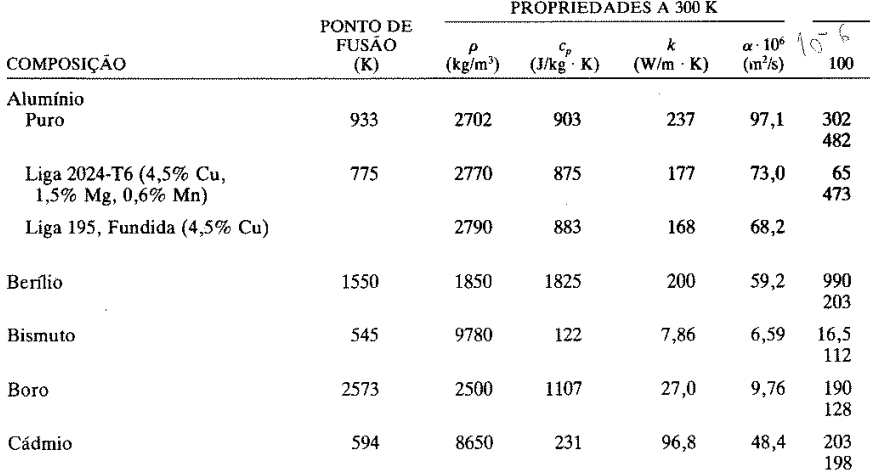
\includegraphics[width=14cm]{figuras/metalProps.jpg}
    \fonteproprioautor
\end{figure}

Isolando o Tb chegamos ao resultado de:
\begin{equation}
    {Tb}={\frac{T1 -T\infty}{{R1}+{R2}}}-{T1} = \SI{109.989}{\degreeCelsius}
\end{equation}

\section{Determinar a taxa de transferência de calor de cada tipo de aleta (qa)}\label{sec:prob1}

